\chapter{Using DashAR}
\label{chap:results}

\begin{center}
    ``Our greatest weakness lies in giving up. The most certain way to succeed is always to try just one more time.'' \\
    - Thomas A. Edison \cite{Gelb2008}
\end{center}

\par Now that the design and development background of the DashAR System has been established, the actual utilization and release of the system can be discussed.

\section{HUD Interface}
    \par After the development phase, the DashAR System's \gls{hud} interface resulted in two major versions. The first interface, as seen in Figure \ref{fig:dasharhuduiversion1}, featured angled trays and widgets, with circular widgets all being the same size. For Figure \ref{fig:dasharhuduiversion1}, it should be noted that the figure is an edited version of the \gls{hud}, for a video presentation. There is no viable option to record the \gls{xr} glasses displays directly. Therefore, this representation of the \gls{hud} must be generated manually. Figure

    \begin{figure}[h!]
        \vspace{0.5cm}
        \centering
        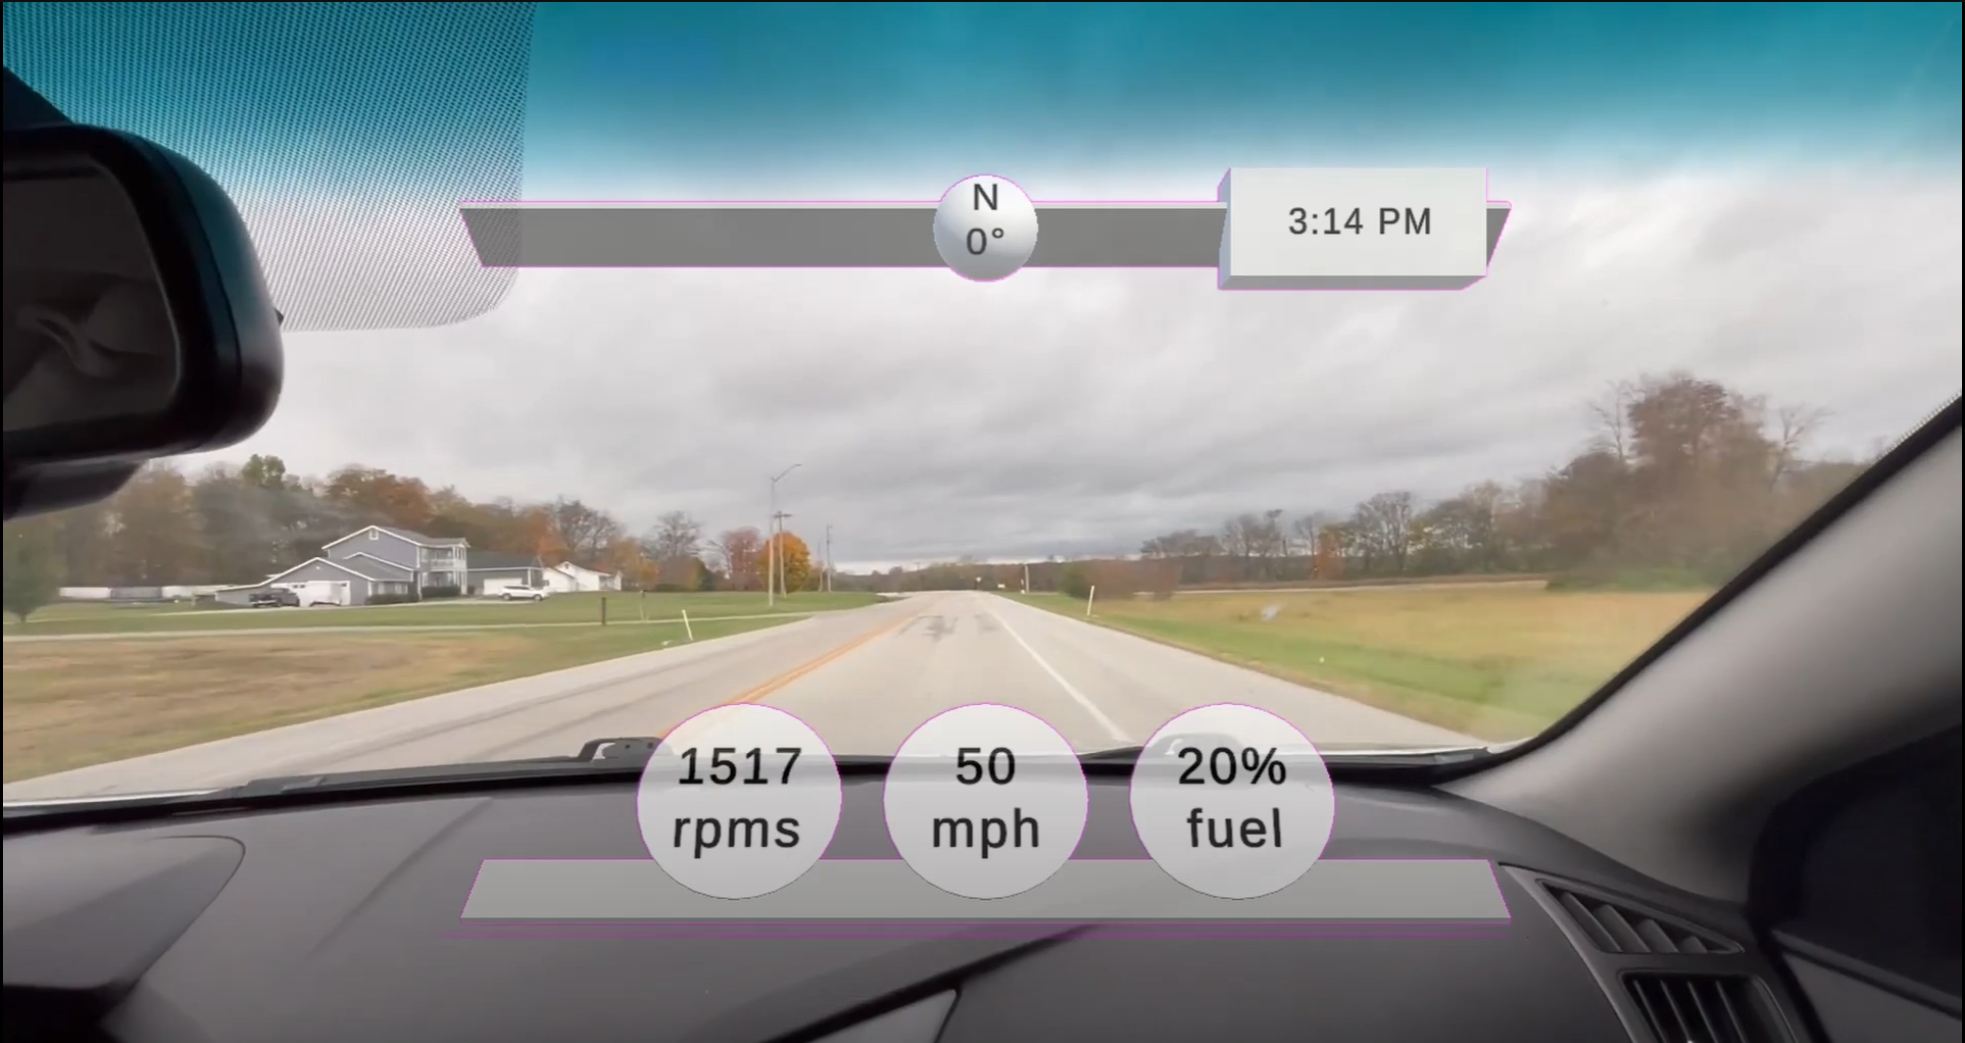
\includegraphics[scale=0.3]{./Support/Images/DashAR-UIVersion1.png}
        \caption{DashAR HUD UI (First Iteration) in Use}
        \label{fig:dasharhuduiversion1}
    \end{figure}

    \begin{figure}[h!]
        \vspace{0.5cm}
        \centering
        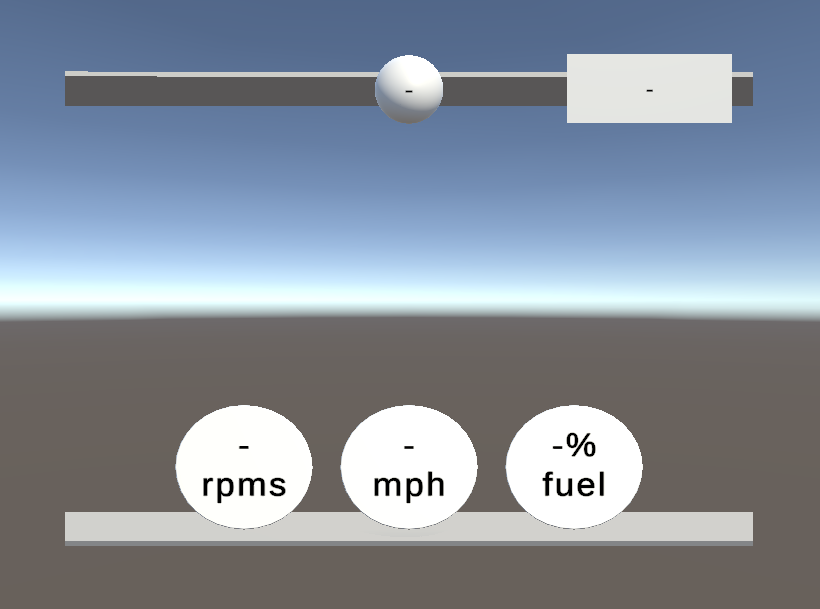
\includegraphics[scale=0.5]{./Support/Images/DashAR-UIVersion1-Unity.png}
        \caption{DashAR HUD UI (First Iteration) in Unity}
        \label{fig:dasharhuduiversion1unity}
    \end{figure}

    \begin{figure}[h!]
        \vspace{0.5cm}
        \centering
        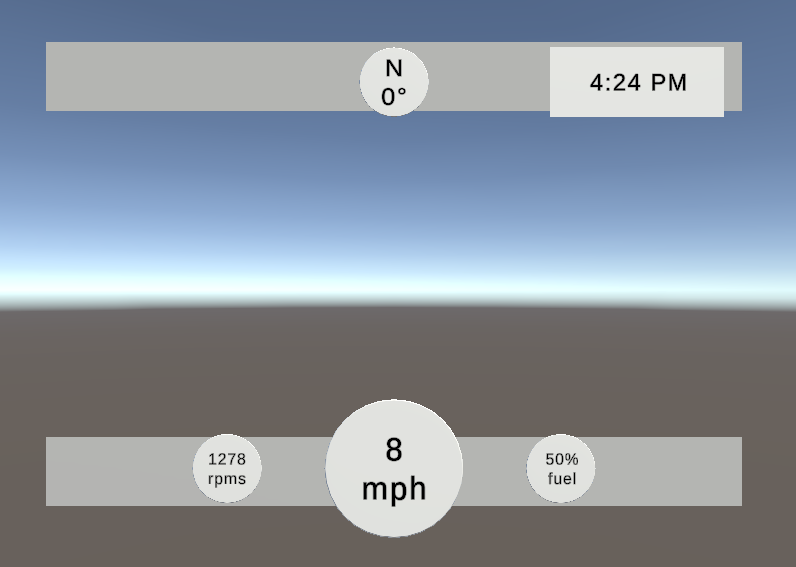
\includegraphics[scale=0.5]{./Support/Images/DashAR-UIVersion2-Unity.png}
        \caption{DashAR HUD UI (Second Iteration) in Unity}
        \label{fig:dasharhuduiversion2unity}
    \end{figure}

    \begin{figure}[h!]
        \vspace{0.5cm}
        \centering
        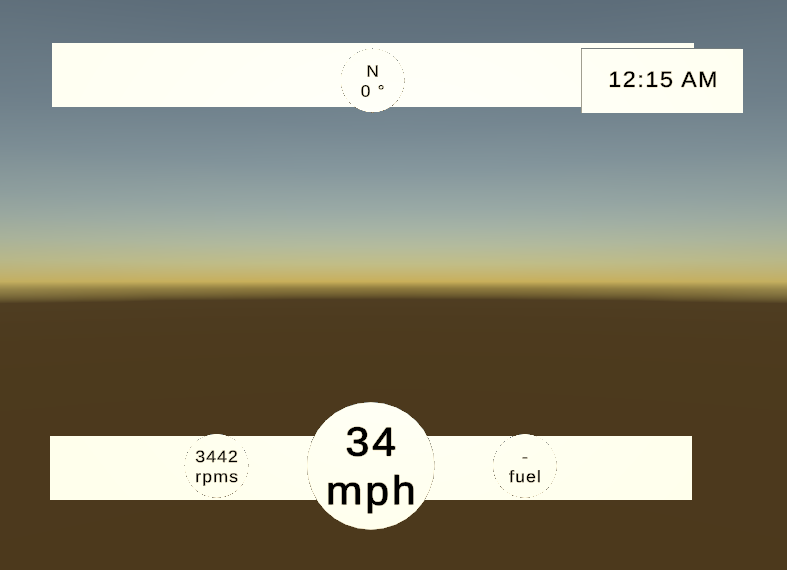
\includegraphics[scale=0.5]{./Support/Images/DashAR-UIVersion2-Dynamic-Unity.png}
        \caption{DashAR HUD UI (Dynamic Generation) in Unity}
        \label{fig:dasharhuduiversion2dynamicunity}
    \end{figure}

\section{Expenses}
    \par At the time of this research, the entire DashAR System can be built for \$777.00, in \glspl{usd}, using off-the-shelf components.

    \begin{table}[]
        \centering
        \caption{DashAR Pricing per Component}
        \label{tab:dasharpricing}
        \begin{tabular}{ll|l|}
            \hline
            \multicolumn{1}{|c|}{Subsystem} & \multicolumn{1}{c|}{Component} & \multicolumn{1}{c|}{Cost (in USD)} \\ \hline
            \multicolumn{1}{|l|}{\gls{ics}}       & Raspberry Pi 5 \cite{CanaKitCorporation2025}                 & 80.00                              \\ \hline
            \multicolumn{1}{|l|}{\gls{ics}}       & Raspberry Pi 5 Power Supply \cite{CanaKitCorporation2025a}   & 12.00                              \\ \hline
            \multicolumn{1}{|l|}{\gls{ics}}       & OBDII-to-USB Interface \cite{Amazon2025}         & 35.00                              \\ \hline
            \multicolumn{1}{|l|}{\gls{ar}}        & XREAL Air 2 Pro \cite{Amazon2025b}                & 400.00                             \\ \hline
            \multicolumn{1}{|l|}{\gls{ar}}        & XREAL Beam Pro \cite{Amazon2025a}                & 200.00                             \\ \hline
            \multicolumn{1}{|l|}{All}       & Surge Protector \cite{Amazon2025c}                & 10.00                              \\ \hline
            \multicolumn{1}{|l|}{All}       & Power Inverter (12V to 120V) \cite{Amazon2025d}   & 40.00                              \\ \hline
                                            &                                & 777.00                             \\ \cline{3-3}
            \end{tabular}
    \end{table}

    \par

\section{Testing}
    \par This section discusses testing scenarios, including UX testing.

